\documentclass[discrete.tex]{subfiles}

\begin{document}
  \section{Задача о кратчайшем остовном дереве. Алгоритм Прима с.208}
  \begin{definition}
    Дерево, являющееся частичным графом связного графа называется остовным деревом
  \end{definition}

  \begin{task}
    Пусть каждой дуге j графа $<M,N,T>$ сопоставлено неотрицательное число $l[j]$, именуемое длиной этой дуги. Требуется построить такое остовное дерево $<M,N',T>$, у которого сумма длин дуг $\sum_{j \in N'} l[j]$ была бы минимальна
  \end{task}

  \begin{alg}[Прима]

  \end{alg}

  \begin{theorem}

  \end{theorem}

  \begin{proof}

  \end{proof}
  \begin{figure}[H]
          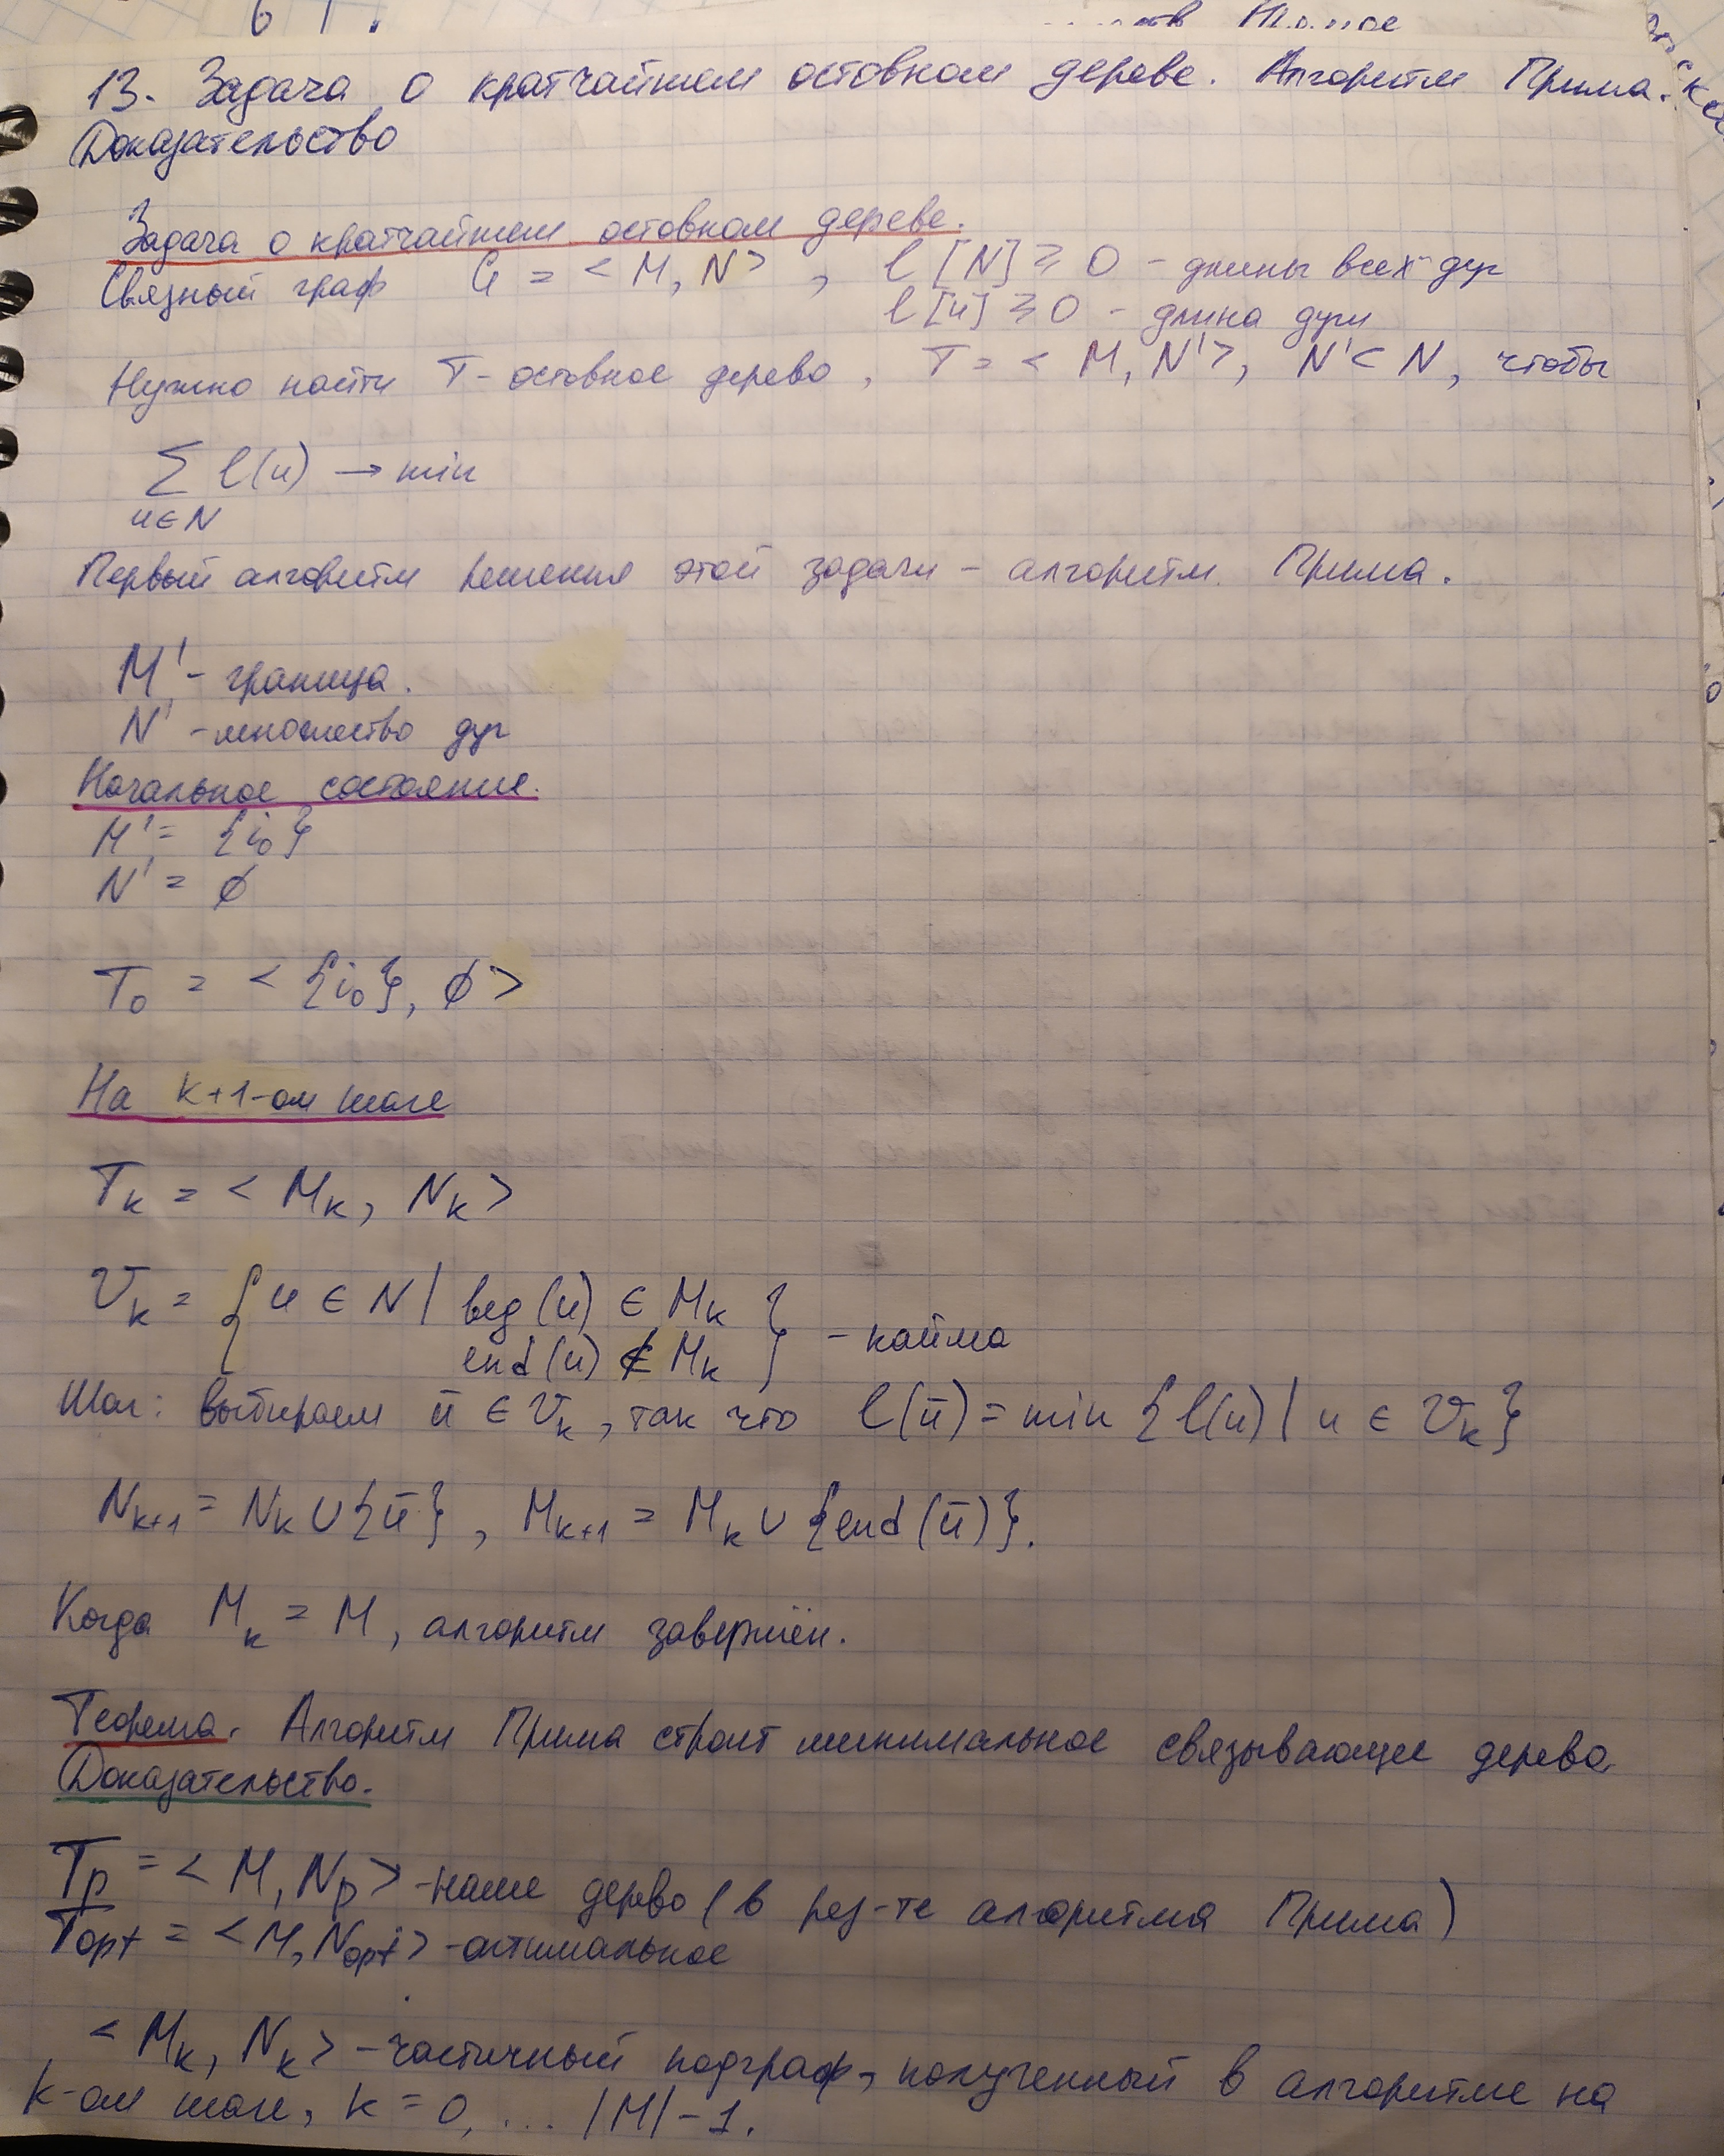
\includegraphics[width=10cm]{pics/43_1}
          \centering
  \end{figure}
  \begin{figure}[H]
          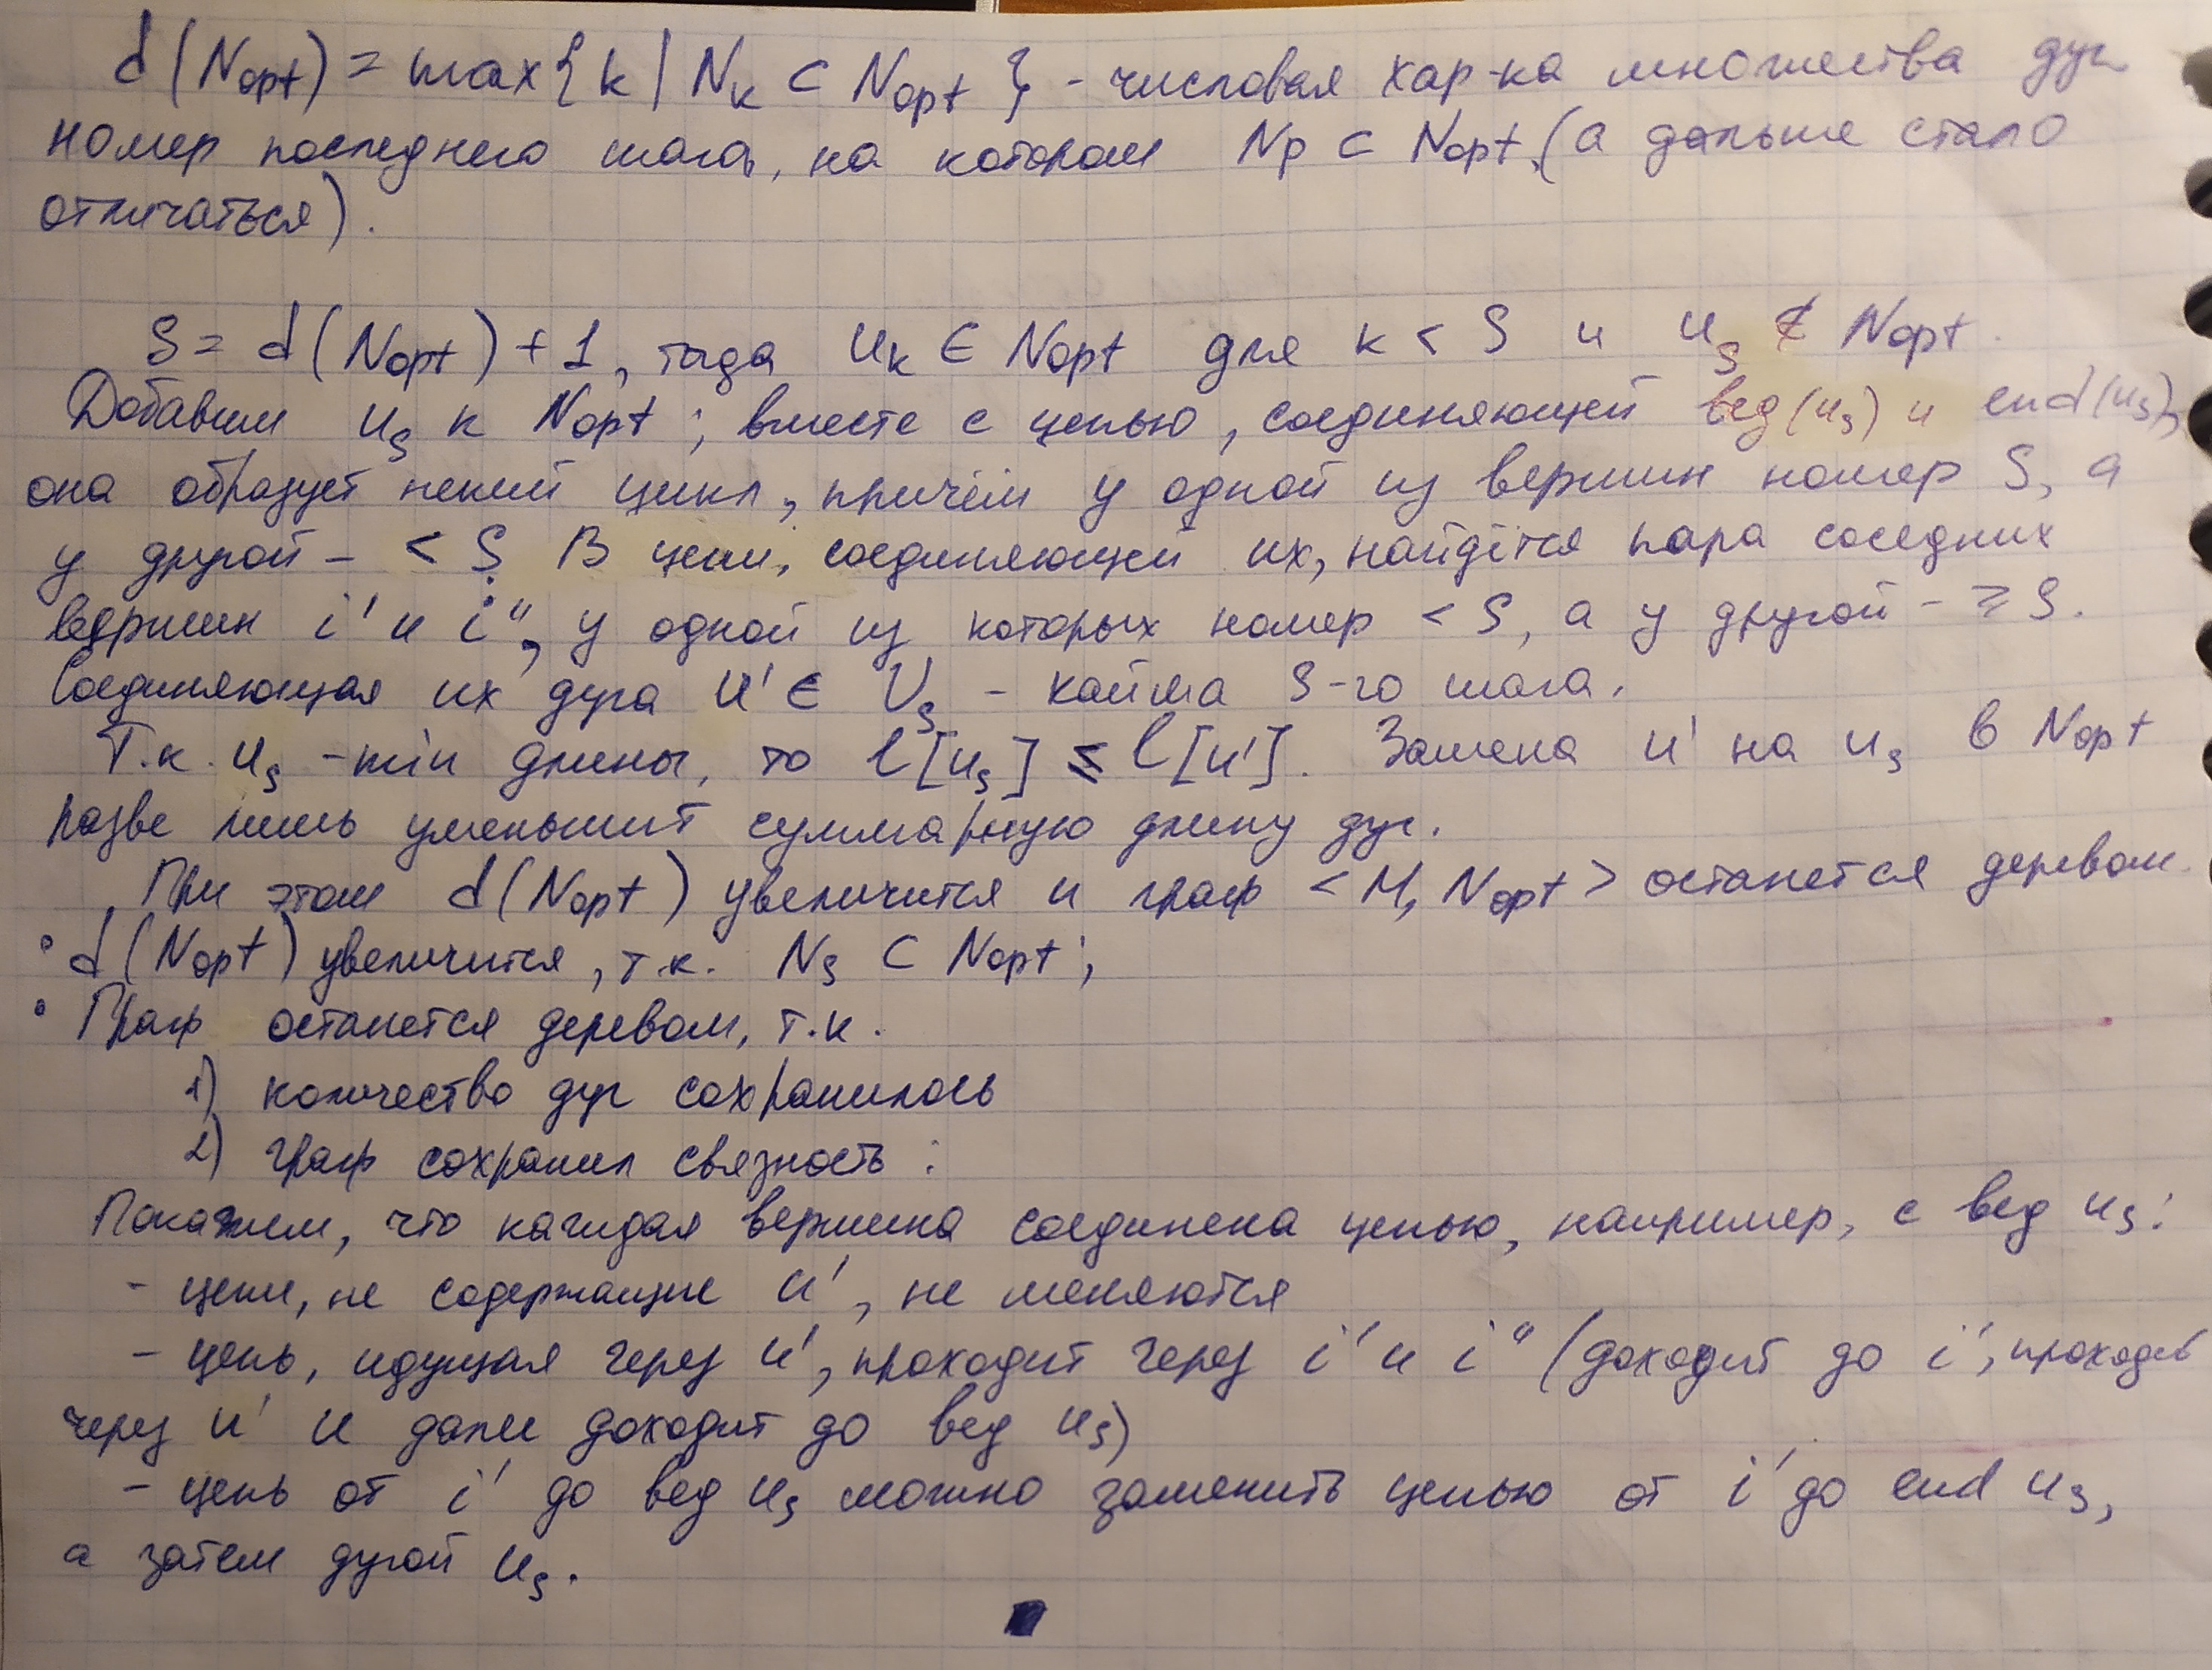
\includegraphics[width=10cm]{pics/43_2}
          \centering
  \end{figure}
\end{document}
